\documentclass[10pt,twocolumn]{article}

% Self-contained Overleaf draft. Replace the document class and geometry with
% the official conference style at submission time; the section files and
% figure paths do not otherwise depend on a particular template.
\usepackage[letterpaper,margin=0.72in,columnsep=0.24in]{geometry}
\usepackage{amsmath,amssymb,booktabs,microtype,multirow}
\usepackage{graphicx}
\usepackage[hidelinks]{hyperref}
\usepackage{xcolor}
\usepackage{enumitem}
\usepackage{siunitx}
\usepackage{cleveref}

\definecolor{fqgreen}{RGB}{0,158,115}
\definecolor{fqorange}{RGB}{230,159,0}
\definecolor{fqblue}{RGB}{0,114,178}
\newcommand{\system}{\textsc{FlagQuantum}}
\newcommand{\todo}[1]{\textcolor{red}{[TODO: #1]}}
\newcommand{\devnote}[1]{\textcolor{fqblue}{[Development evidence: #1]}}

\title{\system: Differentiable Sharded Quantum Simulation\\
for Multi-GPU and Multi-Node Training}
\author{Anonymous Authors}
\date{}

\begin{document}
\maketitle

\begin{abstract}
Quantum machine-learning workloads require both exact quantum-state evolution
and gradients through parameterized circuits, but the memory cost of exact
statevectors grows exponentially and a forward-only distributed simulator does
not complete the training loop.  We present \system, a PyTorch-native quantum
AI runtime organized around one circuit intermediate representation and
backend-independent execution plans.  This paper evaluates its first completed
distributed backend: an amplitude-sharded exact-statevector engine with
sharded forward execution, explicit reverse-mode gradients, owner-sharded
optimizer state, communication-aware wire placement, and topology-aware
multi-node routing.

On one eight-A800 node, a fixed 28-qubit differentiable training workload
achieves \(6.70\times\) end-to-end speedup and \(6.17\times\) backward speedup
from one to eight GPUs.  Across two nodes and 16 A800 GPUs, a 30-qubit
scientific training workload achieves \(5.42\times\) end-to-end and
\(6.46\times\) backward speedup relative to one GPU.  A matched 35-qubit
workload produces a measured single-A800 out-of-memory failure but completes
multiple optimizer steps on 16 GPUs without full-state reconstruction.
Raw-gradient errors remain below \(9\times10^{-8}\) in the reported studies.
A frozen 24-qubit, depth-8 workload measured with five warmups and 30 samples
achieves \(1.644\times\) end-to-end speedup on eight GPUs, with a bootstrap
95\% confidence interval of \([1.636,1.653]\).

The wider \system architecture reserves the same IR, planner, gradient, and
training contracts for matrix-product-state (MPS) and tensor-network (TN)
backends.  Their optimized distributed evaluations are intentionally left as
explicit paper modules rather than claimed from incomplete evidence.
\end{abstract}

\section{Introduction}

Exact statevector simulation is a useful substrate for quantum algorithm
development and quantum machine learning, but a complex64 state requires
\(2^{n+3}\) bytes before accounting for gradients, checkpoints, optimizer
state, and temporary buffers.  Distributing only the forward pass is
insufficient: training additionally requires a sharded reverse pass,
parameter-gradient ownership, optimizer updates, and synchronization that do
not reconstruct the full state on one rank.

\system is designed as a unified quantum AI system rather than a collection of
unrelated simulators.  A single circuit IR feeds local and distributed
statevector, MPS, and TN execution plans.  PyTorch is the primary training
interface; each backend is responsible for honest memory, communication, and
gradient semantics.  The statevector backend is the first backend for which we
have completed the full multi-GPU evidence loop.  This paper therefore makes a
focused systems claim about distributed differentiable statevectors while
leaving explicit extension points for later MPS and TN results.

This draft supports the following contributions:
\begin{itemize}[leftmargin=*,nosep]
  \item An exact amplitude-sharded statevector runtime whose forward and
  reverse passes preserve one logical workload across ranks.
  \item A communication-aware execution strategy combining wire placement,
  cross-shard gate packing, bounded exchange workspaces, and topology-aware
  rank-bit ordering.
  \item A differentiable training path with owner-sharded optimizer state and
  a packed parameter collective that replaces per-parameter broadcasts.
  \item An evaluation spanning single-GPU kernel performance, one-node
  1/2/4/8-GPU scaling, two-node 16-GPU training, raw-gradient correctness,
  and a measured single-GPU-OOM/multi-GPU-completion capacity case.
  \item A backend contract that will place optimized MPS and TN execution
  under the same IR, planning, training, and evidence model.
\end{itemize}

\paragraph{Current submission status.}
The implementation demonstrates the core systems capability, but this draft
does not hide remaining evaluation work.  The 1/2/4/8/16 matrix must be rerun
on one final code revision with a uniform long-sample protocol, and system
profiles must add GPU activity, kernel counts, communication time, effective
bandwidth, overlap, and rank imbalance.  \Cref{sec:roadmap} makes these gates
explicit.

\section{FlagQuantum Architecture}
\label{sec:architecture}

\subsection{One IR, multiple simulation backends}

The user constructs parameterized circuits through one \system API.  The IR
retains gate order, wire dependencies, parameter identity, observables, and
backend-independent training semantics.  A planner then selects a local or
distributed backend and emits memory, communication, gradient, and placement
plans.

\begin{figure}[t]
  \centering
  \fbox{\parbox{0.94\columnwidth}{
  \centering
  \textbf{Unified FlagQuantum IR and PyTorch training API}\\[2mm]
  \(\downarrow\) execution / memory / communication / gradient plans\\[1mm]
  \begin{tabular}{ccc}
  \textbf{Statevector} & \textbf{MPS} & \textbf{Tensor network}\\
  completed evidence & reserved module & reserved module
  \end{tabular}\\[1mm]
  \(\downarrow\) local GPU, multi-GPU, multi-node execution
  }}
  \caption{Planned system architecture.  This submission's measured systems
  results cover the statevector backend.  MPS and TN occupy first-class
  backend positions but receive results only after their own distributed
  gradient and evidence gates pass.}
  \label{fig:architecture}
\end{figure}

\subsection{Execution and evidence semantics}

We call an execution \emph{sharded} only when one logical state is partitioned
across ranks.  Replicated circuits are useful for throughput but are not
capacity expansion.  Every measured result records world size, local world
size, node count, rank placement, per-rank memory, communication, gradient
semantics, and validation blockers.  Single-device execution remains a
separate fast path and does not initialize distributed machinery.

\subsection{Reserved MPS backend module}
\label{sec:mps-placeholder}

\todo{After MPS optimization, add site/bond partitioning, truncation-gradient
policy, boundary-adjoint exchange, canonicalization strategy, and owner-local
optimizer state.  The evaluation slot should include bond-dimension scaling,
accuracy versus exact statevector, one-device crossover, multi-GPU capacity,
and a training workload that exceeds one GPU.}

\subsection{Reserved tensor-network backend module}
\label{sec:tn-placeholder}

\todo{After TN optimization, add contraction planning, slicing and intermediate
ownership, reverse contraction, path-search cost, and multi-node reduction.
The evaluation slot should separate exact from approximate contraction and
report contraction FLOPs, largest intermediate, slicing overhead, accuracy,
and communication.}

\section{Distributed Differentiable Statevectors}
\label{sec:method}

\subsection{Amplitude and wire sharding}

For \(P=2^p\) ranks, each rank owns \(2^{n-p}\) complex amplitudes.  Gates on
local address bits execute without communication.  Gates touching a sharded
address bit exchange only the required partner region.  The planner chooses
sharded wires using gate activity and subgroup alignment, then orders selected
rank bits to move frequently active communication onto cheaper topology tiers.

\subsection{Forward optimizations}

The local fast path groups independent one-qubit regions, composes immutable
single-qubit matrices once, caches constants on device, and uses
\system-owned Triton kernels for common RY/RZ and general complex \(2\times2\)
regions.  Consecutive CX operations are fused into a direct-address
permutation.  For a cross-shard CX, a sharded control becomes a rank-conditional
local operation, while a sharded target exchanges only the control-one
half-space.

\subsection{Sharded reverse mode}

The reverse pass reuses the distributed state layout and applies adjoint gates
in reverse order.  Exchange buffers are chunked and retained in a bounded
workspace.  A fused VJP kernel computes input-state adjoints and parameter
contributions without materializing full-state Jacobians.  Raw parameter
gradients are compared against a one-GPU reference before a cross-world result
is accepted.

\subsection{Optimizer ownership and synchronization}

Parameter \(i\) is assigned to owner rank \(i\bmod P\).  Only the owner retains
Adam state and updates that parameter.  A naive implementation issued one
broadcast per scalar parameter.  \system instead packs owner values, masks
non-owned entries, reconstructs the full vector with one all-reduce, and writes
it back with a foreach operation while preserving the original tensor
identities and autograd references.

\section{Experimental Methodology}
\label{sec:methodology}

\paragraph{Hardware.}
All reported GPU measurements use NVIDIA A800-SXM4-80GB GPUs.  Single-node
experiments use up to eight GPUs.  Multi-node experiments use two eight-GPU
hosts.  \todo{Add CPU, driver, CUDA, NCCL, interconnect, NIC, switch, and
topology inventory from the final unified rerun.}

\paragraph{Workloads.}
The evaluation uses Full-width Linear, Ring, and Brickwork parameterized
circuits with complex64 amplitudes.  Reported training steps include
differentiable forward execution, explicit adjoint backward, owner-local Adam,
and parameter synchronization.  The 30q and 35q scientific cases use a
one-layer Full-width Linear HEA; the frozen significance case uses 24 qubits,
eight layers, 376 gates, and 192 trainable parameters.

\paragraph{Timing and statistics.}
CUDA work is synchronized around timed regions.  The frozen long-sample point
uses five warmups and 30 measured samples.  Speedup confidence intervals use
10,000 independent bootstrap resamples of the median ratio.  Retained
optimization-campaign results with fewer samples are shown as development
measurements without confidence intervals.

\paragraph{Correctness.}
Distributed values, raw parameter gradients, and updated parameters are
checked against the one-GPU reference when it fits.  Capacity evidence requires
a measured single-device OOM and multi-GPU training completion without a full
state reconstruction.

\section{Evaluation}
\label{sec:evaluation}

\subsection{Same-host scaling}

\begin{figure*}[t]
  \centering
  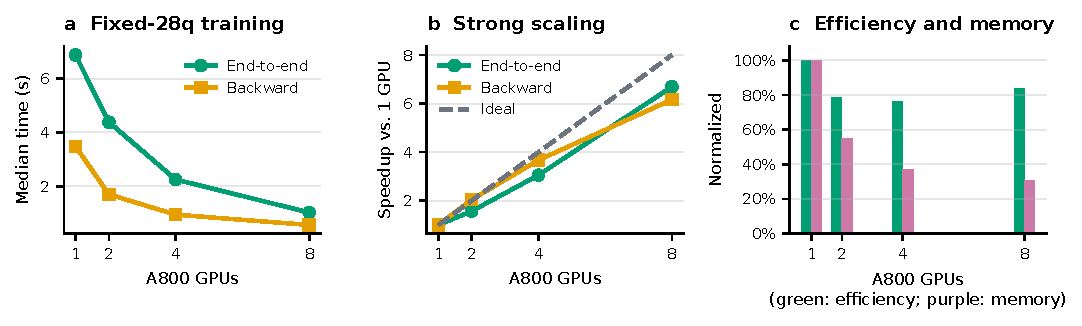
\includegraphics[width=\textwidth]{fig1_scaling.pdf}
  \caption{Strong scaling of differentiable exact-statevector training on one
  eight-A800 node.  The fixed 28-qubit Full-width Linear HEA uses complex64
  amplitudes, RY rotations, directed CX entanglers, explicit sharded adjoint
  backward, and owner-sharded Adam.  Eight GPUs achieve \(6.70\times\)
  end-to-end and \(6.17\times\) backward speedup; distributed raw gradients
  match the one-GPU reference within \(5.96\times10^{-8}\).  These are retained
  matched campaign measurements; the final submission should replace them with
  a unified-version 30-sample 1/2/4/8/16 matrix.}
  \label{fig:scaling}
\end{figure*}

\Cref{fig:scaling} shows that fixed-workload training benefits from amplitude
sharding on one node.  End-to-end median time falls from 6.876\,s on one GPU to
1.027\,s on eight GPUs.  Backward falls from 3.480\,s to 0.564\,s.  The
corresponding parallel efficiencies are 83.7\% and 77.1\%.

\subsection{Where the improvement comes from}

\begin{figure*}[t]
  \centering
  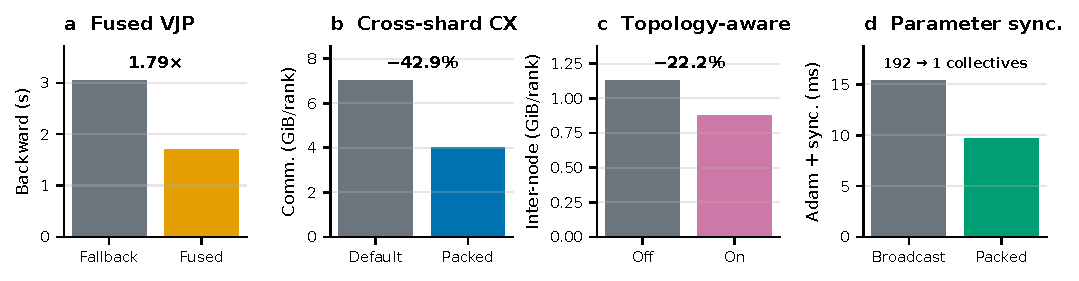
\includegraphics[width=\textwidth]{fig2_optimization_mechanisms.pdf}
  \caption{Ablations of compute, communication, topology, and optimizer
  synchronization.  The fused VJP improves two-GPU backward by \(1.79\times\);
  cross-shard CX packing reduces Ring backward communication by 42.9\%;
  topology-aware rank-bit ordering reduces two-node inter-node backward traffic
  by 22.2\%; and packed parameter synchronization replaces 192 broadcasts with
  one collective while reducing Adam plus synchronization from 15.35\,ms to
  9.67\,ms.}
  \label{fig:ablations}
\end{figure*}

The ablations in \Cref{fig:ablations} isolate four distinct layers of the
system.  They show that local operator throughput alone is insufficient:
address-aware communication, physical topology, and the classical optimizer
boundary all materially affect the training step.

\subsection{Multi-node training and capacity}

\begin{figure*}[t]
  \centering
  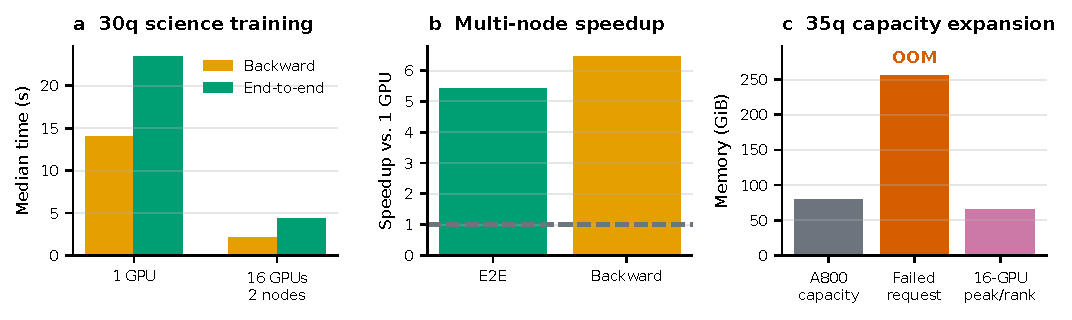
\includegraphics[width=\textwidth]{fig3_training_and_capacity.pdf}
  \caption{Multi-node acceleration and capacity expansion.  A 30q scientific
  training step decreases from 23.45\,s on one A800 to 4.32\,s on 16 A800 GPUs
  across two nodes.  A matched 35q workload triggers a measured OOM on one
  79.25-GiB A800 when requesting a 256-GiB state allocation, whereas 16 GPUs
  complete multiple training steps with 64.61\,GiB peak allocation per rank.
  The 256-GiB bar is the failed allocation request, not resident memory.}
  \label{fig:capacity}
\end{figure*}

The 30q result in \Cref{fig:capacity} demonstrates time-to-solution improvement
for an end-to-end training workload that also fits on one GPU.  The distinct
35q case demonstrates capacity expansion.  Neither result substitutes for the
other: a credible distributed training system must show both.

\subsection{Statistical significance and external context}

\begin{figure*}[t]
  \centering
  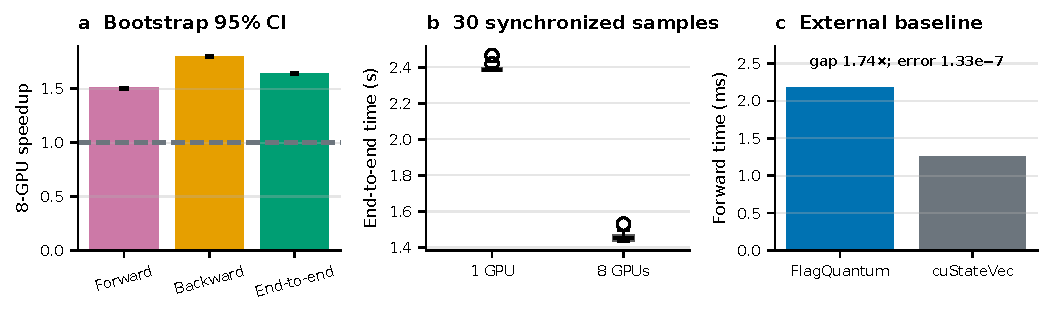
\includegraphics[width=\textwidth]{fig4_statistics_and_external_baseline.pdf}
  \caption{Long-sample evidence and isolated external context.  The frozen
  24q/depth-8 workload uses five warmups and 30 synchronized samples.
  Eight-GPU end-to-end speedup is \(1.644\times\), with bootstrap 95\% CI
  \([1.636,1.653]\); value and raw-gradient errors are
  \(1.12\times10^{-8}\) and \(2.24\times10^{-8}\).  On the same A800 and a
  matched 20q forward workload, \system measures 2.185\,ms versus 1.259\,ms for
  cuStateVec, with \(1.33\times10^{-7}\) final-state error.  cuStateVec is an
  isolated forward-only benchmark and is not a \system dependency.}
  \label{fig:statistics}
\end{figure*}

\begin{figure*}[t]
  \centering
  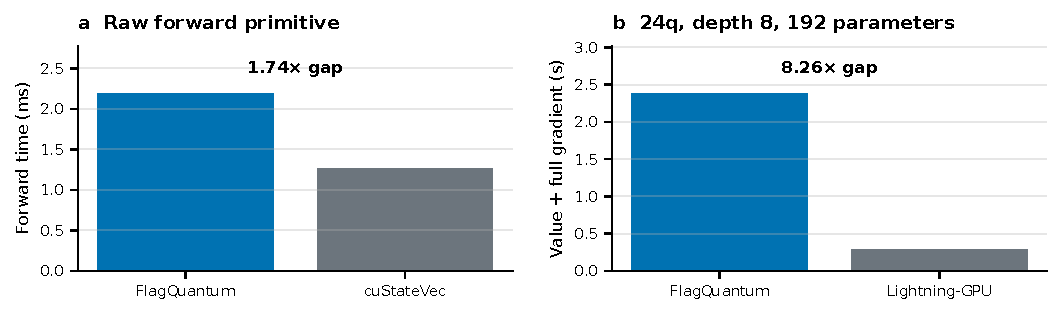
\includegraphics[width=\textwidth]{fig5_differentiable_external_baseline.pdf}
  \caption{Two external baselines with deliberately separated semantics.
  The raw 20q forward comparison measures 2.185\,ms for \system and
  1.259\,ms for cuStateVec.  The differentiable comparison executes the same
  24q/depth-8, 376-gate, 192-parameter workload on one A800 and includes the
  expectation value plus the complete adjoint gradient: \system measures
  2.376\,s versus 0.288\,s for PennyLane Lightning-GPU, an \(8.26\times\)
  gap.  Value and maximum-gradient errors are \(1.86\times10^{-8}\) and
  \(2.24\times10^{-8}\).  Lightning-GPU is a cuQuantum-backed external
  system; neither it nor cuQuantum is a \system runtime dependency.}
  \label{fig:differentiable-external}
\end{figure*}

\section{MPS and Tensor-Network Expansion Plan}
\label{sec:mps-tn}

The intended paper can grow in one of two honest ways:
\begin{enumerate}[leftmargin=*]
  \item \textbf{Focused statevector paper.} Submit after completing the
  statevector gates in \Cref{sec:roadmap}.  MPS/TN remain architecture
  extensions and future work.
  \item \textbf{Full FlagQuantum paper.} Delay submission until MPS and TN each
  demonstrate a differentiable distributed workload, a capacity or crossover
  result, correctness, and a matched systems ablation.  Add one methods
  subsection and one evaluation figure per backend.
\end{enumerate}

The second option has a larger product story but a higher evidence burden.
Adding incomplete MPS/TN numbers would weaken rather than strengthen the
statevector contribution.

\section{Related Work}

\todo{Add verified citations and a comparison table covering exact
statevector simulators, GPU quantum libraries, differentiable simulators,
distributed quantum simulation, MPS training, and TN contraction systems.
Separate library primitives from end-to-end differentiable training systems,
and distinguish replicated throughput from one-state sharding.}

\section{Limitations}

The current evidence covers complex64 A800 systems, two nodes, and the reported
gate/workload families.  External comparisons are currently single-device:
raw cuStateVec for forward execution and PennyLane Lightning-GPU for matched
adjoint differentiation.  The measured \(8.26\times\) differentiable gap shows
that \system's distributed scaling and capacity results do not imply
single-GPU kernel parity with a mature cuQuantum-backed implementation.  The
statevector method remains exponentially expensive and does not replace
approximate MPS/TN methods for low-entanglement regimes.  Current figures do
not yet report GPU activity, communication time, overlap, or effective network
bandwidth.  Abrupt multi-node worker loss under independent elastic agents
also remains distinct from clean application-level fault handling.

\section{Submission Roadmap}
\label{sec:roadmap}

\paragraph{P0: required before a main-track submission.}
\begin{enumerate}[leftmargin=*,nosep]
  \item Freeze one final revision and rerun the identical 28q workload on
  1/2/4/8 GPUs and two-node 16 GPUs with five warmups and at least 30 samples.
  \item Add bootstrap confidence intervals to every primary scaling point and
  report rank-level distributions, not only maxima.
  \item Profile kernel count, SM/GPU activity, communication time, achieved
  NVLink/RoCE bandwidth, compute--communication overlap, and rank imbalance.
  \item Rerun all four mechanism ablations on the final revision with matched
  sample counts and disclose negative or neutral results.
  \item Retain raw logs and exact hardware/software inventory, and package a
  one-command artifact workflow.
\end{enumerate}

\paragraph{P1: strongly recommended.}
\begin{enumerate}[leftmargin=*,nosep]
  \item Sweep qubits \(\{24,26,28,30\}\), depths \(\{8,16,32\}\), and
  cross-shard-gate fractions to identify the single-/multi-GPU crossover.
  \item Extend the matched PennyLane Lightning-GPU adjoint baseline from the
  completed single-A800 point to distributed execution after validating a
  CUDA-aware MPI installation; otherwise document why no like-for-like
  distributed run is available.
  \item Evaluate a third node count or a second interconnect topology.
  \item Add a planner validation showing that automatic backend/layout choices
  select the measured side of each crossover.
\end{enumerate}

\paragraph{Reserved MPS gates.}
Distributed forward and backward, boundary-gradient communication,
bond-dimension/accuracy tradeoff, single-GPU crossover, capacity completion,
and an end-to-end training workload.

\paragraph{Reserved TN gates.}
Contraction planning, slice/intermediate ownership, reverse contraction,
largest-intermediate memory, communication/reduction cost, accuracy, and an
end-to-end differentiable workload.

\section{Conclusion}

\system demonstrates that exact-statevector distribution can preserve the
entire quantum-training loop rather than stopping at forward simulation.
Current results establish promising multi-GPU scaling, real multi-node
training, and capacity expansion with raw-gradient correctness.  The remaining
work is primarily evaluation unification and systems profiling, not fabrication
of missing functionality.  MPS and TN remain first-class positions in the
architecture and will be added only when their own evidence reaches the same
standard.

\end{document}
